\documentclass[11pt]{article}

\usepackage[margin=0.82in]{geometry}
\usepackage{amsmath,amssymb,booktabs,tabularx,array,graphicx}
\usepackage{url}
\usepackage[hidelinks]{hyperref}

\title{Coordinate-Matched Delayed Residual Learning for Discrete Position-Loop Compensation: A Frozen-Controller Simulation Study}
\author{}
\date{Internal manuscript draft --- 24 October 2026; evidence status: not qualified}

\newcommand{\clip}{\operatorname{clip}}
\newcommand{\Cset}{\mathcal{C}}
\newcommand{\Qmetric}{Q}
\newcommand{\NOpred}{\textsc{NoPred}}
\newcommand{\Cfive}{\textsc{C5}}
\newcommand{\DSSM}{\textsc{DSSM}}
\newcommand{\KAN}{\textsc{KAN}}

\begin{document}
\maketitle

\begin{abstract}
This paper reports a frozen simulation evaluation of a coordinate-matched, delayed residual-compensation controller for a discrete multirotor position loop. The candidate, C5-M110, uses a pretrained feature encoder, a linear output head, and a causal update based on a completed 10-ms velocity interval. Across 48 prespecified TEST scenes and six methods (288 audited method-scene records), C5 has mean 0--20-s three-dimensional position RMSE $Q=12.155996$ mm, compared with 18.619575 mm for the traceable baseline B; it wins 46 scenes and loses two. Its paired scene-bootstrap mean difference against B is $-6.463579$ mm (95\% descriptive interval $[-9.114101,-4.171965]$ mm). Against a matched ablation that removes only the delayed-prediction gradient, the difference is smaller ($-0.505912$ mm; interval $[-0.682267,-0.327261]$ mm), and the T2 interval crosses zero. A finite-path posterior $Q$ bound is separately instantiated on all 72 development trajectories; it is conditional on the observed path and is not a prior plant-stability or future-performance guarantee. The test package retains all losses and discloses recovery and historical-exposure limitations. These results support a narrow simulation claim for one frozen controller, plant, model seed, and scene set; they do not establish real-flight performance, cross-seed generalization, or broad novelty for online residual adaptation.
\end{abstract}

\section{Introduction}
A learned residual can change both the applied input and the command-filter states that define the tracking error. Consequently, a lower regression loss for one residual coordinate does not alone determine physical position error. In the fixed loop studied here, applied compensation $u$ and the discrete physical forcing $d_0$ satisfy
\begin{equation}
  u-d_0 = \epsilon_M + M r_f, \qquad
  \epsilon_M := u-d_M, \quad d_M := d_0+M r_f,
  \label{eq:physical-coordinate}
\end{equation}
where $r_f$ is the command-filter realization difference. The term $M r_f$ remains in the physical forcing. Fitting the coordinate-matched target $d_M$ more closely therefore does not, by itself, guarantee a smaller position error.

This paper asks a restricted implementation question: in one frozen discrete simulation loop, how does a fixed PCF-coordinate mask and a causal delayed-prediction gradient compare with matched alternatives? We report the complete TEST48 comparison and preserve each scene-level loss. The relevant contribution is an explicitly timed, coordinate-matched implementation and its fixed-design evaluation, alongside a conditional finite-path analysis. We do not claim a new general composite-learning principle, a first use of interval labels, a first projected update, or a first neural residual controller.

\section{Related work and contribution boundary}
Neural-Fly combines learned features and adaptive linear coefficients for agile flight in strong winds~\cite{oconnell2022neuralfly}; integral concurrent learning uses interval data under its own finite-excitation assumptions~\cite{parikh2019integral}. Discrete-time adaptive controllers with causal error models and high-order tuners provide a distinct analytical setting~\cite{fisher2023discrete}. DATT uses a learned trajectory-tracking architecture with a disturbance-estimation channel~\cite{huang2023datt}, while command-filtered adaptive fuzzy quadrotor control has also been reported~\cite{zhao2024commandfilter}. The full text for the cited 2024 command-filtered paper was not available for equation-level comparison in this review, so no theorem-level priority claim is made.

A closer precedent is Jiang et al.'s composite-learning neural controller for dual-arm robots with relative motion~\cite{jiang2022composite}. Their continuous-time command-filtered backstepping design combines an RBF network, tracking and exponentially weighted historical-prediction terms in one weight-adaptation law, and a projection that keeps weights within a norm ball. Under their partial persistent-excitation condition, their theorem establishes convergence of tracking and weight errors to small neighborhoods and bounded contact-force error for that dual-arm system. Thus command filtering, neural approximation, tracking-plus-prediction composite adaptation, and weight projection are established ingredients; none is claimed here as new. C5 instead uses a fixed pretrained encoder and linear head in a discrete quadrotor position loop, a fixed PCF mask, a completed 10-ms velocity-increment label, and a single elementwise box projection after combining the current tracking term, leakage, and previous-interval prediction gradient. These are implementation-level differences, not a transfer of Jiang et al.'s PPE assumption or theorem to this quadrotor.
Two recent works further bound any broad novelty statement about online adaptation. Altawaitan and Atanasov combine an offline multi-step neural dynamics model with online low-rank, second-order parameter adaptation for predictive control~\cite{altawaitan2026adapting}. Pan et al. describe alternating online residual-dynamics learning and policy optimization through differentiable simulation~\cite{pan2026learningfly}. The present system differs in its fixed nominal controller, pretrained fixed encoder, adaptive linear output head, PCF-coordinate target, and completed-interval update. This structural distinction is not evidence of priority. We make no claim to be the first to combine offline learning with online adaptation or to perform online residual learning for quadrotors.

The study-specific questions are whether the fixed mask $M=\operatorname{diag}(1,1,0)$ and the delayed-prediction term improve this configured loop relative to the tested alternatives, and whether the implemented projected update admits a useful finite-path bound. The empirical mechanism evidence is limited to matched comparisons; it does not establish counterfactual causality outside this fixed simulation design.

\section{Controller and evaluation protocol}
\subsection{Coordinate-matched delayed update}
The simulation uses fixed nominal position backstepping and attitude controllers, command-filter realization, plant, actuators, and nominal parameters $C_0,J_0$. It assumes ideal, noiseless full-state Euler-angle feedback. The learner receives no wind or morphology/configuration variable. Let $a_{\mathrm{req}}=a_{\mathrm{nom}}-u$ be requested acceleration, $a_f$ the acceleration implied by the filtered command, and $r_f=a_{\mathrm{req}}-a_f$. An auxiliary PCF state evolves at the 1-ms simulation step as
\begin{equation}
  \eta[n+1]=e^{-4\Delta t}\eta[n]
       +\frac{1-e^{-4\Delta t}}{4}r_f[n],
  \qquad \eta[0]=0, \quad \Delta t=1~\mathrm{ms}.
\end{equation}
For the fixed diagonal mask $M$, C5 uses $M=\operatorname{diag}(1,1,0)$, modified surface $s_M=s-M\eta$, and reference acceleration $a_M=a_{\mathrm{req}}-Mr_f$. Thus the $x$ and $y$ coordinates use the PCF correction while $z$ retains the nominal coordinate. The mask is fixed for every scene; it is not selected from wind or scene identity.

C5 uses the locked DSSM14 encoder (14 input channels and a 32-step window) and its unit-normalized 33-dimensional feature vector $\phi$. Its linear head $W\in\mathbb{R}^{33\times3}$ begins from the same trained weights $W_0$ in every scene; model seed 2026102001 and selected step 60000 are fixed. Offline training targets the physical acceleration residual $a_{\mathrm{actual}}-a_{\mathrm{req}}$. Online learning instead uses velocity increments relative to $a_M$, so the online label includes the PCF coordinate shift $Mr_f$ in general.

Updates occur at $n_q=320+10q$, $q=0,\ldots,1967$. At event $q$, the controller first applies the output of current weights,
\begin{equation}
  u_q=\beta_q\clip(W_q^\top\phi_q,-3,3),
  \qquad \beta_q=\min\!\left(\frac{(n_q+1)\Delta t}{1.8~\mathrm{s}},1\right),
\end{equation}
where clipping is componentwise and $u_q$ is in $\mathrm{m}/\mathrm{s}^2$. Only at event $q\geq1$ is the preceding interval label available. With $h=10\Delta t=0.01$~s, it is
\begin{equation}
  y_{q-1}=\frac{v[n_q]-v[n_{q-1}]
          -\Delta t\displaystyle\sum_{i=n_{q-1}}^{n_q-1}a_M[i]}{h}.
  \label{eq:interval-target}
\end{equation}
This is an interval-average residual from sampled velocity, not an instantaneous disturbance measurement. The update retains $\phi_{q-1}$ for its delayed gradient and applies one joint box projection:
\begin{align}
  W_{q+1}&=\Pi_{\Cset}(W_q-G_q), \qquad
  \Cset=[-60,60]^{33\times3}, \\
  G_q&=0.12\beta_q\phi_q s_{\mathrm{eff},q}^{\top}
       +0.00002W_q
       +0.01\phi_{q-1}(W_q^{\top}\phi_{q-1}-y_{q-1})^{\top}, \quad q\geq1,
  \label{eq:update}
\end{align}
where $s_{\mathrm{eff},q}=\clip(s_M[n_q],\pm[7,8,10])$. At $q=0$, the delayed-prediction term is zero because no completed prior interval exists. The output is held between events; the newly updated weights do not change the output already applied at that event.

\subsection{Methods and matched ablations}
The six evaluated methods are B (baseline), DSSM14, KAN14, C5-M110, Frozen W0, and NoPred. The freeze ablation retains the pretrained encoder and $W_0$ but disables online weight updates; it is not a no-network comparison. The NoPred ablation removes only the delayed-prediction coefficient and retains the C5 initialization, encoder, PCF, mask, interval target, readiness, event clock, tracking update, leakage, clipping, and projection. The two corrected external comparators are reported under their frozen method identities; their labels do not imply algorithmic equivalence to C5.

\subsection{Scenes, metric, and inference}
The development evidence uses 72 DEV24+VAL48 scenes, each a 20-s, 1-ms-step simulation. On DEV72, C5 has mean $Q=11.558928$ mm versus 17.058081 mm for B (64 wins, 8 losses); Frozen W0 has 34.910909 mm and NoPred 12.110171 mm. C5 beats NoPred in 54/72 scenes, but the T2 paired interval crosses zero. These data are development context and are not pooled with the independent test.

\noindent\textbf{Development-stage mask contrast.}\par The single-factor development comparison changed the C3/M111 mask to C5/M110 while holding the remaining frozen configuration constant. Across the same 72 DEV scenes, M110 had a scene-equal mean $Q=11.558928371$ mm versus $11.759244913$ mm for M111 (paired mean change $-0.200316542$ mm); M110 was lower in 53/72 scenes (19 losses). In the high-frequency DEV group, mean $Q$ was lower by $0.440679$ mm. This is development-stage selection evidence only: TEST48 did not include an independent C3/M111 mask-only arm. TEST48 includes C5-M110 and NoPred but not C3/M111, so the full TEST C5-versus-B improvement is not attributed to the mask.

The frozen TEST48 contains 48 scene identities, with 16 scenes per task T1--T3, evaluated with all six methods for 288 audited method-scene records. Each simulated run lasts 20 s at 1-ms steps. W09--W14 form the high-frequency group (18 scenes); W15 is the no-wind group (3 scenes). The candidate, model identity, normalizer, scene set, and scoring rules were frozen before TEST. No TEST outcome was used to select or tune C5.

For scene $i$, the primary metric is the full-horizon, scene-level three-dimensional position RMSE
\begin{equation}
  Q_i=\sqrt{\frac{1}{N}\sum_{n=0}^{N-1}
      \|p_i[n]-p_{i,\mathrm{ref}}[n]\|_2^2},
  \qquad N=20{,}000,
  \label{eq:q}
\end{equation}
using samples $n=0,\ldots,19{,}999$ and excluding the terminal state at 20 s. Group means weight scenes equally. Paired wins use unrounded $Q_i$ in metres and a $10^{-12}$-m tie tolerance; separate 1- and 10-$\mu$m sensitivity counts are retained. Confidence intervals use 10,000 paired physical-scene bootstrap resamples within each group (seed 2026102301), with common indices across comparator contrasts and linear 2.5\%/97.5\% quantiles. They are descriptive for this fixed simulation design, have no multiplicity correction, and do not support cross-training-seed inference.

\section{Finite-path posterior bound}
For $q\geq1$, define $\psi_q=\phi_{q-1}$, $\rho=0.01$, $\ell_q(W)=\tfrac12\|W^\top\psi_q-y_{q-1}\|_2^2$, $g_q=\psi_q(W_q^\top\psi_q-y_{q-1})^\top$, and write the actual update gradient as $G_q=\rho g_q+b_q$, where $b_q$ contains the tracking and leakage terms. For a comparator $U\in\Cset$ fixed before the path, define $D_q=\|W_q-U\|_F^2$, $\bar W_{q+1}=W_q-G_q$, $Z_q=\Pi_{\Cset}(\bar W_{q+1})$, and the ideal projection residual $R_q^{\mathrm{ideal}}=Z_q-\bar W_{q+1}$. Let $\delta_q=W_{q+1}^{\mathrm{actual}}-Z_q$ represent the stored floating-point update. For $1\leq m\leq1967$,
\begin{equation}
\begin{aligned}
&2\rho\sum_{q=1}^{m}[\ell_q(W_q)-\ell_q(U)]
+\rho\sum_{q=1}^{m}\|\psi_q^\top(W_q-U)\|_2^2 \\
&\leq D_1-D_{m+1}+\sum_{q=1}^{m}\|G_q\|_F^2
-2\sum_{q=1}^{m}\langle b_q,W_q-U\rangle_F
-\sum_{q=1}^{m}\|R_q^{\mathrm{ideal}}\|_F^2 \\
&\quad+\sum_{q=1}^{m}\left[2\langle\delta_q,Z_q-U\rangle_F+\|\delta_q\|_F^2\right].
\end{aligned}
\label{eq:path-bound}
\end{equation}
The terms due to tracking, leakage, projection, and floating-point residual are retained. The inequality does not imply that the right-hand side is small.

The historical-output bridge bounds the sum of squared residuals for the weights that actually produced prior outputs by $2P+2L^2J$, where $P$ is the accumulated delayed prediction loss, $J=\sum_q\|W_q-W_{q-1}\|_F^2$, and $L\geq\max_q\|\phi_q\|_2$. The physical-forcing bridge retains the ramp, interval-target variation, output clipping, and $Mr_f$ terms. Combined with the checked sampled position recursion and its 800/200 convolution gains, this yields a posterior finite-path bound on $Q$.

This limited bound was instantiated for all 72 audited DEV trajectories using $L=1+10^{-9}$ and a per-element $10^{-10}$ numerical residual envelope. The bound-to-observed-$Q$ ratios range from 3.740385 to 31.331274; the largest recomputed post-projection discrepancy is $2.220446\times10^{-16}$. These checks use ordinary double precision, not outward-rounded interval certification. They verify the conditional inequality on completed paths; they do not establish a prior Plant-domain invariant, closed-loop stability, parameter convergence, future performance, or superiority to B. The older local prior ISS/domain certificate remains unproved/infeasible and is not replaced by this distinct posterior path bound. This analysis is DEV-only and is not presented as a bound instantiated on TEST48.

\section{TEST48 results}
\subsection{Primary error and paired comparisons}
Table~\ref{tab:groupmeans} reports scene-equal mean $Q$. C5 is lower than B on the full TEST48, the high-frequency group, and W15, while its advantage over NoPred is modest. All six methods completed the simulations; the meaning and limits of process identity are described in Section~\ref{sec:limitations}.

\begin{table}[t]
\centering
\small
\caption{Mean full-horizon three-dimensional position RMSE $Q$ (mm); lower is better.}
\label{tab:groupmeans}
\begin{tabular}{lrrrrrr}
\toprule
Group ($n$) & B & DSSM14 & KAN14 & C5-M110 & Frozen W0 & NoPred \\
\midrule
All TEST48 (48) & 18.619575 & 13.052592 & 16.068314 & 12.155996 & 36.157333 & 12.661908 \\
High-frequency W09--W14 (18) & 11.693191 & 12.358965 & 14.242926 & 11.005986 & 38.665891 & 11.408303 \\
No-wind W15 (3) & 6.755625 & 6.762105 & 8.926326 & 5.527405 & 19.795262 & 6.755205 \\
\bottomrule
\end{tabular}
\end{table}

Across all scenes, C5 beats B in 46/48 scenes, DSSM14 in 41/48, KAN14 in 48/48, Frozen W0 in 48/48, and NoPred in 36/48, with no ties at the primary tolerance. Winner counts are unchanged at 1- and 10-$\mu$m tie thresholds for every comparator. The C5--B mean paired difference is $-6.463579$ mm (95\% interval $[-9.114101,-4.171965]$ mm). Table~\ref{tab:contrasts} shows all TEST48 comparator contrasts. The intervals are descriptive paired-scene bootstrap intervals, not independent samples of trained controllers.

\begin{table}[t]
\centering
\small
\caption{TEST48 paired scene-equal difference, C5 minus comparator, and stored descriptive 95\% bootstrap interval (mm). W/L/T counts use the $10^{-12}$-m tie tolerance.}
\label{tab:contrasts}
\begin{tabular}{lrrr}
\toprule
Comparator & Mean difference & 95\% interval & W/L/T \\
\midrule
B & $-6.463579$ & [$-9.114101,-4.171965$] & 46/2/0 \\
DSSM14 & $-0.896596$ & [$-1.147851,-0.661642$] & 41/7/0 \\
KAN14 & $-3.912318$ & [$-4.333520,-3.535123$] & 48/0/0 \\
Frozen W0 & $-24.001337$ & [$-25.554333,-22.463413$] & 48/0/0 \\
NoPred & $-0.505912$ & [$-0.682267,-0.327261$] & 36/12/0 \\
\bottomrule
\end{tabular}
\end{table}

Against B, C5 wins 15/16 T1 scenes, 15/16 T2 scenes, and all 16 T3 scenes. The paired mean differences and intervals are $-6.547302$ mm (T1, 95\% interval $[-11.054773,-2.845688]$), $-6.145502$ mm (T2, $[-10.979514,-2.179595]$), and $-6.697934$ mm (T3, $[-11.183719,-2.986744]$). The high-frequency group has 16 wins and two losses against B; W15 has three wins and no losses. The corresponding paired differences are $-0.687205$ mm (HF, $[-1.046213,-0.322537]$) and $-1.228220$ mm (W15, $[-1.382350,-1.026594]$). W15 contains only three scenes.

The NoPred contrast is smaller than the C5--B difference. In T2, C5 minus NoPred is $-0.152312$ mm with a descriptive 95\% interval $[-0.436521,0.100665]$ mm, which crosses zero. The observed all-scene interval for C5--NoPred is below zero, but these fixed-design intervals do not establish a universal benefit from the delayed-prediction term. The matched freeze comparison is much larger: C5 wins all 48 scenes against Frozen W0, while Frozen W0 retains the same pretrained representation and weights.

\subsection{Retained losses and visual summaries}
All C5 losses against every comparator are retained in the paired CSV and listed here. Against B, the two losses are \texttt{T1\_C14\_W09} (+0.106685 mm) and \texttt{T2\_C14\_W12} (+1.162507 mm). Against DSSM14, losses are \texttt{T2\_C00\_W14}, \texttt{T2\_C06\_W04}, \texttt{T2\_C08\_W06}, \texttt{T2\_C09\_W07}, \texttt{T2\_C11\_W09}, \texttt{T2\_C14\_W12}, and \texttt{T3\_C11\_W12}. C5 has no losses against KAN14 or Frozen W0. Against NoPred, losses are \texttt{T1\_C03\_W14}; \texttt{T2\_C00\_W14}, \texttt{T2\_C02\_W00}, \texttt{T2\_C06\_W04}, \texttt{T2\_C08\_W06}, \texttt{T2\_C09\_W07}, \texttt{T2\_C10\_W08}, \texttt{T2\_C11\_W09}, \texttt{T2\_C12\_W10}, \texttt{T2\_C14\_W12}; and \texttt{T3\_C09\_W10}, \texttt{T3\_C11\_W12}. Scene IDs share the prefix \texttt{DL1018\_TEST\_}. The full comparator-level metric and provenance rows are supplied with this draft.

\begin{figure}[t]
\centering
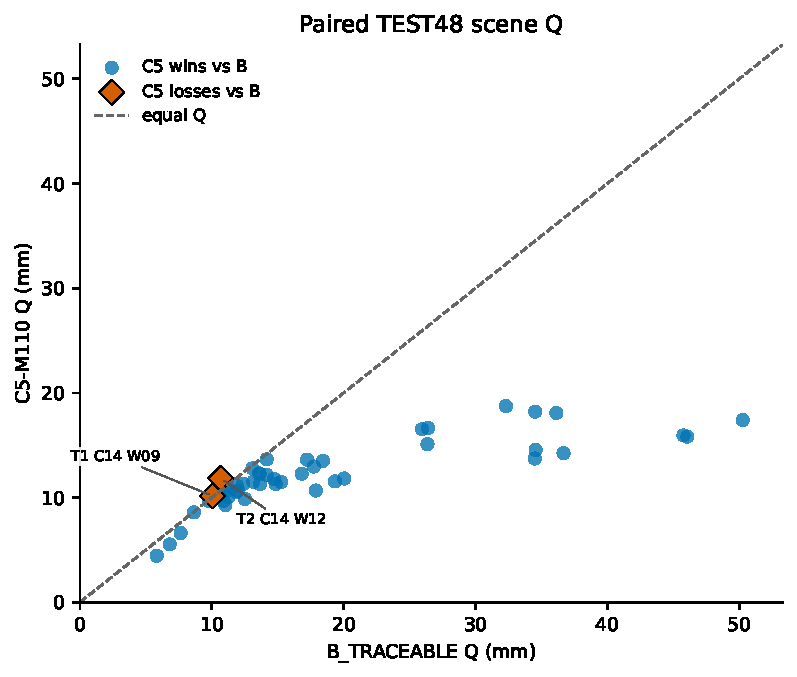
\includegraphics[width=0.78\linewidth]{figures/fig1_paired_Q_C5_vs_B.pdf}
\caption{Paired C5--B scene-level $Q$ values. The two C5 losses are marked in the source figure and remain in the reported totals.}
\label{fig:scatter}
\end{figure}

\begin{figure}[t]
\centering
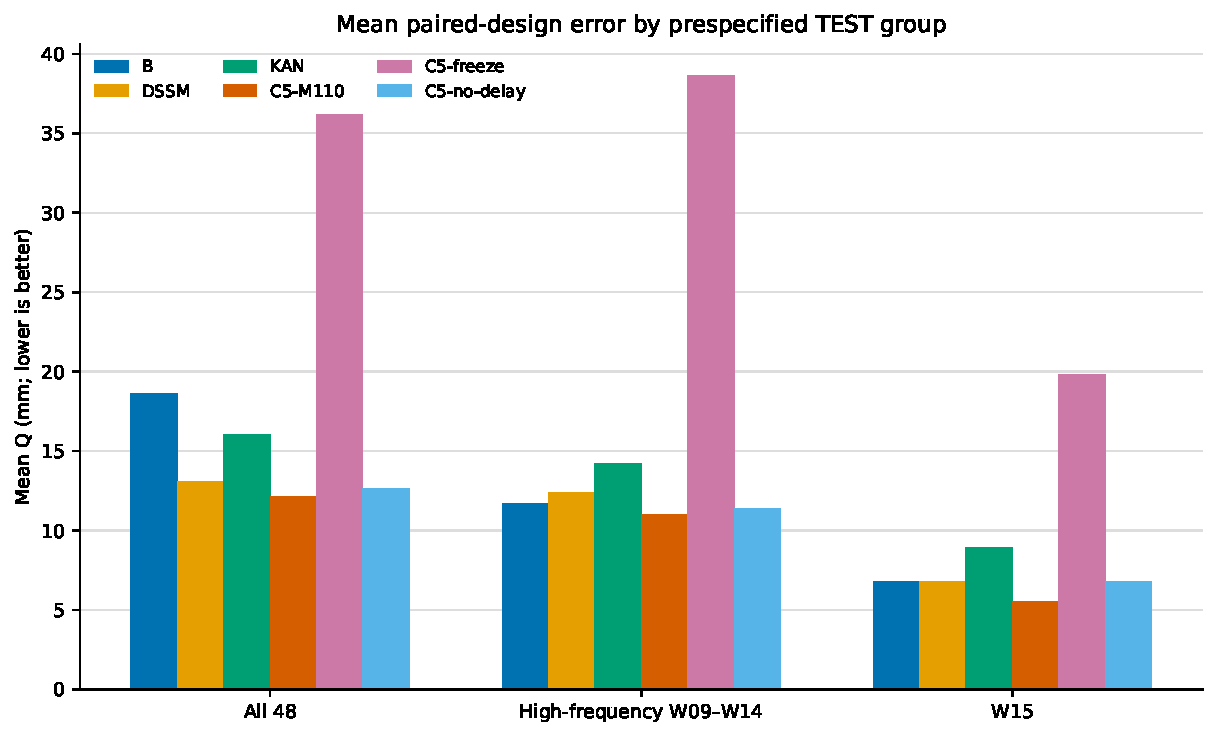
\includegraphics[width=0.92\linewidth]{figures/fig2_grouped_Q_comparison.pdf}
\caption{Mean $Q$ by all TEST48, high-frequency W09--W14, and no-wind W15 groups for the six evaluated methods.}
\label{fig:groups}
\end{figure}

\begin{figure}[t]
\centering
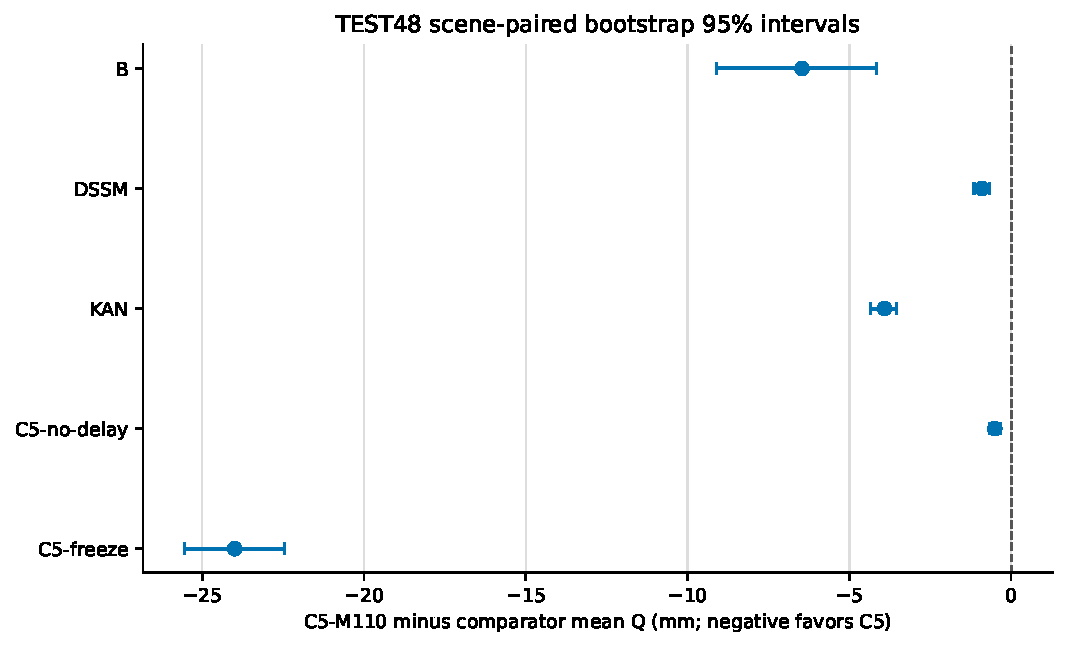
\includegraphics[width=0.88\linewidth]{figures/fig3_paired_bootstrap_CI_ALL48.pdf}
\caption{Paired scene-bootstrap intervals for C5 minus each comparator on ALL48. Negative values favor C5; intervals describe this fixed simulation design.}
\label{fig:ci}
\end{figure}

\subsection{Per-axis, phase, peak, safety, and actuator summaries}
Table~\ref{tab:axis} gives all-scene per-axis RMSE for B and C5 over the full horizon and the 0--5-s and 5--20-s phases. The aggregate three-dimensional $Q$ and per-axis RMSE are distinct summaries. C5's full-horizon 95th-percentile position error is 25.537673 mm versus 36.142788 mm for B; its mean scene peak is 39.294977 mm versus 54.684825 mm. All 288 rows have status STABLE, are complete, and have finite actuator records. No safety-stop row, generalized-output clipping, or motor-saturation fraction was recorded in the supplied statistics. These checks are specific to the audited simulation outputs.

\begin{table}[t]
\centering
\small
\caption{Scene-equal per-axis position RMSE (mm), averaged over the 48 TEST scenes.}
\label{tab:axis}
\begin{tabular}{lrrrrrr}
\toprule
Axis & B 0--20 & C5 0--20 & B 0--5 & C5 0--5 & B 5--20 & C5 5--20 \\
\midrule
$x$ & 11.136377 & 7.652997 & 11.922506 & 10.022417 & 10.472373 & 6.190056 \\
$y$ & 11.986387 & 8.040398 & 10.854196 & 8.949808 & 11.937219 & 7.090964 \\
$z$ & 3.288256 & 2.305569 & 3.667123 & 3.484798 & 3.014994 & 1.617916 \\
\bottomrule
\end{tabular}
\end{table}

\subsection{Controller-call timing}
The audit reports controller-call telemetry separately from the simulated 1-ms plant step. Table~\ref{tab:timing} reports mean call time and the across-scene mean of per-scene ready-call p95/p99 values. Each scene has 19,680 ready calls and 320 nonready calls. The process runs were sequential; JIT effects are included; no operating-system timing isolation was used. The measurement ends before allocation, Plant stepping, or MAT-file saving and is not a full-loop timing test. It therefore does not support a 1-kHz deadline or hard-real-time claim.

\begin{table}[t]
\centering
\small
\caption{Descriptive controller-call timing (ms). Ready-call p95/p99 columns are means of per-scene quantiles.}
\label{tab:timing}
\begin{tabular}{lrrr}
\toprule
Method & Mean call & Ready p95 & Ready p99 \\
\midrule
B & 0.140235 & 0.355545 & 0.544100 \\
DSSM14 & 0.170557 & 0.496776 & 0.730732 \\
KAN14 & 0.132453 & 0.429915 & 0.585944 \\
C5-M110 & 0.134139 & 0.402271 & 0.553006 \\
Frozen W0 & 0.131862 & 0.393762 & 0.537117 \\
NoPred & 0.133162 & 0.394809 & 0.550060 \\
\bottomrule
\end{tabular}
\end{table}

Four prespecified performance checks pass in the stored independent review: at least 41 C5 wins over B (observed 46), all-scene mean below B, high-frequency mean no larger than B, and W15 mean no larger than B. These checks summarize performance only; they do not qualify the complete paper evidence package. The separate evidence checkpoint remains \texttt{NOT\_QUALIFIED} pending contribution review and final reproducibility/release review.

\section{Discussion and limitations}\label{sec:limitations}
The TEST48 result supports a fixed-design simulation statement: the frozen C5-M110 controller had lower mean $Q$ than B in this 48-scene batch, and the paired scene-level differences are recorded with the full loss set. The matched ablation evidence is narrower. C5 is better than NoPred on 36/48 scenes and has a lower mean, but 12 scenes regress, and the T2 bootstrap interval crosses zero. Frozen W0 performs substantially worse in this batch, but the comparison does not establish that a learned representation has no value; it retains the trained weights and exposes the difference between the offline physical target and the PCF-shifted online target.

The benchmark contains one model seed (2026102001, selected step 60000), one fixed simulated plant and actuator model, ideal noiseless full-state Euler-angle feedback, and no real flight. It does not establish cross-seed reliability, sensor-noise robustness, transfer to other plants, or deployment performance. The no-wind group has only three scenes. Timing is descriptive controller-call telemetry under sequential, non-isolated processes, not full-loop or hard-real-time evidence. No formal claim of universal stability, parameter convergence, or future-path error is made.

The original DSSM process history has a specific identity limitation: its natural exit status is UNKNOWN, and one scene (scene32) lacks a runIdentity. The recovered DSSM tail16 has OS0 evidence; the other method blocks have OS0 records. The earlier six-process OS0 gate remains UNMET and is not reclassified by the recovered runs. These limitations do not change the reported Q values, but they constrain process-level provenance claims.

A historical-exposure incident records that two summaries for older TEST scenes were accidentally displayed during an older diagnostic; at the time, overlap with the present TEST48 was UNKNOWN. The record also states that the C5 model and selection in this branch were frozen before the exposure and were not tuned from those summaries. A later metadata-only review compared four old configuration/execution snapshots for the two identified scenes (\texttt{TEST\_C10\_34\_J1} and \texttt{TEST\_C10\_34\_J2}) with the 48 current TEST scenes over 12 shared exogenous fields (2,304 field comparisons). It found no complete match for either old ID among those fields; seven core fields---reference position, velocity and acceleration, arm command, \texttt{arms/rho\_true}, \texttt{arms/rhoDot\_true}, and wind---each matched 0/48 current scenes. The old sources lack \texttt{arms/rho\_hat} and \texttt{arms/rhoDot\_hat}, so complete 14-field equality could not be checked. This review covers only those two IDs and available metadata; it cannot exclude overlap with every historical TEST scene. The exposure incident and its then-UNKNOWN overlap status remain in the record; we do not claim that no historical TEST information was ever seen. The metadata review did not read old report text or historical scores.

\pagebreak
This manuscript remains an internal evidence draft. A parent audit independently checked all 288 rows and 11,232 numeric table cells against the frozen statistics and visually reviewed the grouped figure. That verification supports data transcription, not broader scientific qualification. The manuscript does not claim novelty priority, real-world validation, or a completed evidence gate.

\section{Conclusion}
On the frozen 48-scene simulation set, C5-M110 had lower scene-level $Q$ than B in 46/48 scenes and a lower scene-equal mean $Q$ than each of the five reported comparators. Its advantage over the matched NoPred ablation was smaller and heterogeneous, with 12 losses and a T2 interval crossing zero. We report the complete paired losses, group and phase summaries, bootstrap intervals, timing, and recovery disclosures. Together with the DEV72 finite-path posterior bound, the evidence supports only a narrow claim about this fixed implementation and these simulated paths. It does not establish general adaptive-control novelty, prior Plant stability, future-path performance, cross-seed reliability, or real-flight performance.

\bibliographystyle{plain}
\bibliography{references}

\end{document}
